\section{Evolución unitaria separable $\mcU=U_{1}\otimes U_{2}$}
Consideramos una unitaria $\mcU=U_{1}\otimes U_{2}$ que evoluciona en el tiempo como $\mcU_{t}=(U_{1}\otimes U_{2})^{t}=U_{1}^{t}\otimes U_{2}^{t}$. Retomando la ecuación (\ref{eq:MaxEntSeparable}), el estado efectivo evolucionado, en términos de un multiplicador de Lagrange y la unitaria $V$ que lo relaciona a un estado alineado en $z$ con la misma pureza es
\begin{align*}
    \CG{(U_{1}^{t}\otimes U_{2}^{t})\varrho_{max}(U_{1}^{t}\otimes U_{2}^{t})^{\dag}}&=p\frac{1}{Z_{1}}U_{1}^{t}V e^{-\lambda p \sigma_{z}}V^{\dag}(U_{1}^t)^{\dag}+(1-p)\frac{1}{Z_{2}}U_{2}^{t}Ve^{-\lambda (1-p)\sigma_{z}}V^{\dag}(U_{2}^t)^{\dag}\\
    &=p\frac{1}{Z_{1}}U_{1}^{t}V e^{-\lambda p \sigma_{z}}(U_{1}^tV)^{\dag}+(1-p)\frac{1}{Z_{2}}U_{2}^{t}Ve^{-\lambda (1-p)\sigma_{z}}(U_{2}^tV)^{\dag}\\
\end{align*}
Por un lado, podemos dejar a las unitarias $V$ dentro de las exponenciales, de tal forma que:
\begin{equation}
    \CG{(U_{1}^{t}\otimes U_{2}^{t})\varrho_{max}(U_{1}^{t}\otimes U_{2}^{t})^{\dag}}=p\frac{1}{2}(\Id+U_{1}^{t}(\hat{r}_{\rho}\cdot\vec{\sigma})(U_{1}^{t})^{\dag}\tanh{(-\lambda p)})+(1-p)\frac{1}{2}(\Id+U_{2}^{t}(\hat{r}_{\rho}\cdot\vec{\sigma})(U_{2}^{t})^{\dag}\tanh{(-\lambda (1-p))}).
\end{equation}
El resultado puede verse como las partes que componen al estado efectivo alineado en $z$ evolucionados por una composición de unitarias, que es otra unitaria. Las unitarias $U_{j}$ pueden escribirse como $e^{-i\theta_{j} \hat{n}_{j}\cdot\vec{\sigma}}$, mientras que $V=e^{i\alpha\hat{l}\cdot\vec{\sigma}}$ con $\hat{l}=(\cos{\beta},\sin{\beta},0)$, luego $U_{i}V=e^{i\zeta_{j} \hat{k}_{j}\cdot \vec{\sigma}}$ donde:
\begin{align*}
    \cos{\zeta_{j} }&=\cos{\theta_{j}}\cos{\alpha}-\hat{n}_{j}\cdot \hat{l}\sin{\theta_{j}}\sin{\alpha}\\
    \hat{k}_{j} &=\frac{1}{\sin{\zeta}}(\hat{n}_{j}\sin{\theta_{j}}\cos{\alpha}+\hat{l}\cos{\theta_{j}}\sin{\alpha}-\hat{n}_{j}\times \hat{l}\sin{\theta_{j}}\sin{\alpha})
\end{align*}
Total que la dinámica se ve como
\begin{equation}
    \boxed{V\CG{\varrho_{max}^{z}}V^{\dag} \xrightarrow{\mcU=U_{1}\otimes U_{2}} pW_{1}\Tr_{2}(\varrho_{max}^{z})W_{1}^{\dag}+(1-p)W_{2}\Tr_{1}(\varrho_{max}^{z})W_{2}^{\dag}}.
\end{equation}
Donde $W_{j}=U_{j}V$. Cada parte del estado efectivo se ve rotado de manera diferente. Las partes que se rotan son las partes que surgen al pasar al estado de máxima entropía por la aplicación de grano grueso. Pensando en esto, \notaAd{Regresar a la parte correspondiente: \ref{sec:CG(MaxEnt)}}. Aunque a mi me gusta la forma
\begin{equation}\label{eq:SeparableDynamics}
    \boxed{\rho\xrightarrow{\mcU=U_{1}\otimes U_{2}} p\frac{1}{Z_{1}}U_{1}e^{-\lambda_{3}p\hat{r}_{\rho}\cdot\vec{\sigma}}U_{1}^{\dag}+(1-p)\frac{1}{Z_{2}}U_{2}e^{-\lambda_{3}(1-p)\hat{r}_{\rho}\cdot\vec{\sigma}}U_{2}^{\dag}}.
\end{equation}

Si el estado inicial tiene componente en $z$ nomás
\begin{equation}\label{eq:SeparableZDynamics}
\CG{(U_{1}^{t}\otimes U_{2}^{t})\varrho_{max}(U_{1}^{t}\otimes U_{2}^{t})^{\dag}}=p\frac{1}{Z_{1}}e^{-\lambda p U_{1}^{t}\sigma_{z}(U_{1}^t)^{\dag}}+(1-p)\frac{1}{Z_{2}}e^{-\lambda (1-p)U_{2}^{t}\sigma_{z}(U_{2}^t)^{\dag}}
\end{equation}
Incluyendo el tiempo y haciendo el cambio $t\theta\rightarrow t$, los exponentes dentro de (\ref{eq:SeparableDynamics}) se desarrollan como:
\begin{align*}
    e^{-i\theta \hat{n}\cdot\vec{\sigma}}\sigma_{z}e^{i\theta \hat{n}\cdot\vec{\sigma}}&=(\Id\cos{t}-i\hat{n}\cdot\vec{\sigma}\sin{t})\sigma_{z}(\Id\cos{t}+i\hat{n}\cdot\vec{\sigma}\sin{t})\\
    &=\sigma_{z}\cos^{2}{t}+i[\sigma_{z},\hat{n}\cdot\vec{\sigma}]\sin{t}\cos{t}+(\hat{n}\cdot\vec{\sigma})\sigma_{z}(\hat{n}\cdot\vec{\sigma})\sin^{2}{t}\\
    &=\sigma_{z}+2\sin{t}\qty((n_{x}\sigma_{y}-n_{y}\sigma_{x})\cos{t}+n_{z}(\hat{n}\cdot\vec{\sigma})\sin{t})
\end{align*}
A notar que si $t=0$ no hay evolución. Luego, en el límite $t\ll 1$:
\begin{equation*}
    e^{-i\theta \hat{n}\cdot\vec{\sigma}}\sigma_{z}e^{i\theta \hat{n}\cdot\vec{\sigma}}=\sigma_{z}+2t(n_{x}\sigma_{y}-n_{y}\sigma_{x})
\end{equation*}
\notaAd{Aún tengo que darle interpretación a esto. Si defino $T=\theta^{-1}$ entonces este límite corresponde justamente a $T$ alta. Mañana voy a desarrollar esto como exponencial real de un vector de Pauli. La expresión es la misma que para la exponencial compleja, pero sin unidad imaginaria e intercambiano las funciones trigonométricas por hiperbólicas}

\subsection{El caso $U_{1}=\Id$ o $U_{2}=\Id$}
Retomando a expresión (\ref{eq:SeparableDynamics}), y en virtud de (\ref{eq:PauliVectorExp}), vemos que el estado efectivo inicial $\rho$ puede verse como una combinación de dos operadores con vector de Bloch con dirección $\hat{r}_{\rho}$. El vector de Bloch de $\rho$ se ve modificado al ser una de sus dos componentes (paralelas) rotada. La rotación siendo $U_{1}$ \notaAd{Creo que dependo mucho de las parametrizaciones de Bloch para entender lo que está pasadno, ¿qué sucede en el espacio de operadores de densidad?}. En general:
\begin{equation}\label{eq:SeparableDynamicsUxI}
    \rho\xrightarrow{\mcU=U_{1}\otimes \Id} p\frac{1}{Z_{1}}U_{1}e^{-\lambda_{3}p\hat{r}_{\rho}\cdot\vec{\sigma}}U_{1}^{\dag}+(1-p)\frac{1}{Z_{2}}e^{-\lambda_{3}(1-p)\hat{r}_{\rho}\cdot\vec{\sigma}}
\end{equation}
En términos del vector de Bloch, denotando $r_{A}=p\tan(-p\lambda_{3})$, $r_{B}=(1-p)\tan(-(1-p)\lambda_{3})$, y $O$ la rotación generada por $U_{1}$:
\begin{equation}
    r\hat{r}_{\rho}\xrightarrow{\mcU=U_{1}\otimes \Id}r_{A}O\hat{r}_{\rho}+r_{B}\hat{r}_{\rho}=O(r\hat{r}_{\rho}-r_{B}\hat{r}_{\rho})+r_{B}\hat{r}_{\rho}
\end{equation}\label{eq:SeparableDynamicsUxIBloch}
El resultado es una rotación alrededor de una línea que no pasa por el origen. Notar que una transformación así no tendría por qué mantener a los estados dentro de la esfera de Bloch, por lo que esta debe depender del estado mismo. La traslación tiene una magnitud $r_{B}$ en la dirección opuesta a la del estado, y esta debe hacerse antes de la rotación, para deshacerse después. Así que, aunque esto podría parecer una transformación afín, no lo es, pues depende enteramente del estado.
\subsubsection{Cambio de fase $H=t\sigma_{z}$}
Considérese el hamiltoniano $H=t\sigma_{z}$. La rotación en la esfera debida a la unitaria generada por el hamiltoniano es una alrededor del eje $z$. La representación de esto, y de el resultado general (\ref{eq:SeparableDynamicsUxIBloch}) puede verse en la figura \ref{fig:ZRot}.

\begin{figure}[h!]
    \centering
    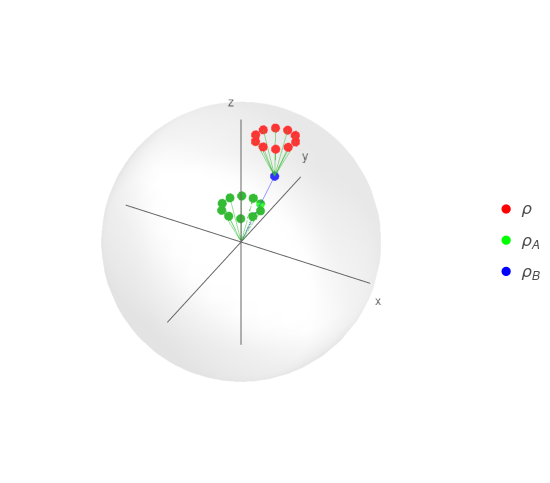
\includegraphics[width=0.6\linewidth]{maxent/figures/Ux1_H=sigmaz_sequence__z=0.9_p=0.4.png}
    \caption{En rojo, la evolución temporal del estado efectivo. En verde y azul, $(r_{A}\hat{r}_{\rho})$ y $(r_{B}\hat{r}_{\rho})$ respectivamente.}
    \label{fig:ZRot}
\end{figure}

En el espacio de operadores de densidad, esto equivale a insertar una fase relativa en el primer subsistema fino. En efecto, ignorando fases globales,
\begin{equation}
    e^{it\sigma_{z}}=\begin{pmatrix}
        1&0\\0&e^{-i2t}
    \end{pmatrix}
\end{equation}
El estado grueso siente el cambio de fase relativa en su primera componente \notaAd{¿Qué son las trazas del MaxEnt?}.
\begin{equation}
    \rho\xrightarrow{\mcU=e^{it\sigma_{z}}\otimes \Id} p\frac{1}{Z_{1}}e^{it\sigma_{z}}e^{-\lambda_{3}p\hat{r}_{\rho}\cdot\vec{\sigma}}e^{-it\sigma_{z}}+(1-p)\frac{1}{Z_{2}}e^{-\lambda_{3}(1-p)\hat{r}_{\rho}\cdot\vec{\sigma}}
\end{equation}


\subsection{Tengo que ver cómo interpreto esta $H=a\sigma_{x}+b\sigma_{y}$}

\subsection{El caso $U_{1}=U_{2}=U$}

Quizá el caso más sencillo. La simetría de la unitaria permite factorizarla:
\begin{align*}
\CG{(U^{t}\otimes U^{t})\varrho_{max}(U^{t}\otimes U^{t})^{\dag}}&=p\frac{1}{Z_{1}}e^{-\lambda p U^{t}\sigma_{z}(U^t)^{\dag}}+(1-p)\frac{1}{Z_{2}}e^{-\lambda (1-p)U^{t}\sigma_{z}(U^t)^{\dag}}\\
&=p\frac{1}{Z_{1}}U^{t}e^{-\lambda p \sigma_{z}}(U^t)^{\dag}+(1-p)\frac{1}{Z_{2}}U^{t}e^{-\lambda (1-p)\sigma_{z}}(U^t)^{\dag}\\
&=U^{t}\qty(p\frac{1}{Z_{1}}e^{-\lambda p \sigma_{z}}+(1-p)\frac{1}{Z_{2}}e^{-\lambda (1-p)\sigma_{z}})(U^t)^{\dag}\\
\end{align*}

\newpage